\section{Mixture of Experts: The Core Concept}

A Mixture of Experts (MoE)~\cite{jacobs1991adaptive,shazeer2017moe,mu2025survey} solves a problem through several specialised networks $E_1,\dots,E_n$ and a small network called the \emph{router} or gate, $G$, which decides how much each expert counts for the current input (Figure~\ref{fig:moe}):
\begin{equation}
\mathrm{MoE}(x)=C\big(\{G_i(x)\cdot E_i(x)\}_{i=1}^{n}\big),
\label{eq:moe}
\end{equation}
where $G_i(x)$ is the contribution of expert $i$ and $C$ is a combination function, classically a sum. Because $G$ takes $x$ as its input, the contributions differ from one input to the next. This is the dynamic behaviour that objective O1 asks for.

\begin{figure}[htbp]
  \centering
  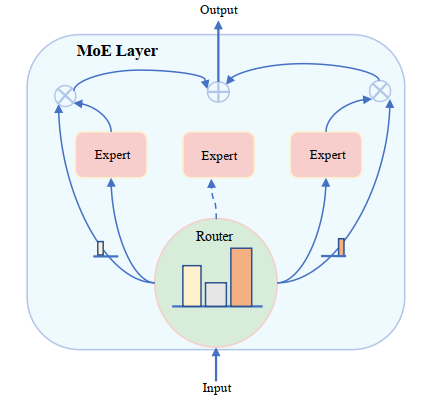
\includegraphics[width=.38\linewidth]{arch_moe.png}
  \caption{A Mixture of Experts layer, from Mu and Lin~\cite{mu2025survey}. The router sets the contribution of each expert for the current input.}
  \label{fig:moe}
\end{figure}

\section{From Output Ensembling to Weight Ensembling}

Equation~\eqref{eq:moe} combines expert \emph{outputs}. Applied directly, it would run every expert for every input, so inference cost would grow with the number of experts and the experts would need a shared output space. Weight-Ensembling Mixture of Experts (WEMoE)~\cite{tang2024wemoe} keeps the router but changes what is combined. An expert is represented by its task vector, the router's values scale those vectors, and the resulting weights are assembled before they are applied (Figure~\ref{fig:we}).

The two forms are not equivalent. For a single linear layer, $(\sum_i w_iW_i)h=\sum_i w_i(W_ih)$, but this equality is lost across non-linear activations and stacked layers. Weight ensembling therefore defines a different function from an ensemble of the experts' outputs. Its potential benefits are one forward pass per input, one checkpoint, and a shared encoder. Its costs are that task vectors must stay stored for every upscaled module, that routers need data to train, and that each input needs its own weights assembled at run time, which can make inference slower even when fewer parameters are stored. Section~\ref{sec:efficiency} measures these costs.

\begin{figure}[htbp]
  \centering
  \resizebox{.62\linewidth}{!}{\begin{tikzpicture}[x=1cm,y=1cm]
  % (a) parameter-level: the gating weight of each expert scales its frozen task vector
  \node[lane] at (-.3,3.05) {(a) Parameter-level combination (implemented)};
  \node[plain] (h) at (.1,-1.25) {$h^{\ell}_i$};
  \node[trn,minimum width=1.2cm] (r) at (1.6,.6) {Router\\$r^{\ell}$};
  \draw[gate] (h.north) |- (r.west);
  \node[frz,minimum width=1.3cm,minimum height=.55cm] (w0) at (4.0,2.4) {$W_0^{\ell}$};
  \draw[gate] (r.east) -- (2.85,.6);
  \foreach \l/\y/\i in {$\tau_1^{\ell}$/1.6/1,$\tau_2^{\ell}$/.8/2,$\tau_E^{\ell}$/-.25/3}{
    \node[frz,minimum width=1.3cm,minimum height=.55cm] (t\i) at (4.0,\y) {\l};
    \node[circle,draw=BrickRed,inner sep=.5pt,font=\scriptsize] (x\i) at (5.4,\y) {$\times$};
    \draw[dict] (t\i) -- (x\i);
    \draw[gate] (2.85,.6) |- (5.4,\y-.39) -- (x\i.south);
  }
  \node[note] at (4.0,.34) {$\vdots$};
  \node[note,anchor=east] at (2.8,-.75) {$w^{\ell}_e(x)$};
  \node[circle,draw=NavyBlue,inner sep=.5pt] (s) at (6.75,.8) {$+$};
  \draw[dict] (w0.east) -| (s.north);
  \foreach \i in {1,2,3} \draw[dict] (x\i.east) -- (s);
  \node[mix,minimum width=2.3cm] (f) at (6.75,-1.25) {$f_{\mathrm{MLP}}\big(h;W^{\ell}(x)\big)$};
  \draw[dict] (s) -- node[note,right] {$W^{\ell}(x)$} (f);
  \draw[flow] (h) -- (f);
  \draw[flow] (f.east) -- ++(.6,0);
  \node[note] at (3.0,-1.75) {one forward pass; per-input weights};
  % (b) output-level
  \draw[black!30,dashed] (8.75,-2) -- (8.75,3.2);
  \node[lane,text=black!70] at (9,3.05) {(b) Output-level combination (not used)};
  \node[plain] (x) at (9.45,.8) {$x$};
  \foreach \l/\y/\i in {$f_1$/2.0/1,$f_2$/1.1/2,$f_E$/-.3/3}{
    \node[dat,minimum width=1.5cm,minimum height=.55cm] (m\i) at (11.25,\y) {Model \l};
    \draw[flow,black!50] (x) -- (m\i.west);
  }
  \node[note] at (11.25,.47) {$\vdots$};
  \node[dat,minimum width=1.75cm] (ls) at (14.2,.8) {$\sum_e G_e(x)\,f_e(x)$};
  \foreach \i in {1,2,3} \draw[flow,black!50] (m\i.east) -- (ls);
  \draw[flow,black!50] (ls.east) -- ++(.5,0) node[right,note] {$\hat y$};
  \node[note] at (12.2,-1.25) {$E$ forward passes; combines logits;\\requires a shared output space};
\end{tikzpicture}
}
  \caption{Parameter-level combination used in this study (a), contrasted with output-level combination (b), which is shown only for reference.}
  \label{fig:we}
\end{figure}

\section{Implementation Flow: From Datasets to Evaluation}
\label{sec:flow}

Figure~\ref{fig:flow} shows the implementation flow in four stages. Stage 1 prepares the five GLUE tasks and divides each official training split into three parts. Stage 2 fine-tunes one expert per task from the pre-trained model, then keeps its task vector and classification head. Stage 3 merges these into one model and trains its routers on the few-shot pool. Stage 4 reports scores on the official validation splits, together with storage and latency. The development split selects the best epoch, the scaling factor $\lambda$ and the best router step, so no selection touches the reported data. Expert weights stay frozen after Stage 2, and only the routers learn in Stage 3.

\begin{figure}[htbp]
  \centering
  \resizebox{.8\linewidth}{!}{% Four-stage flow of the Version 3 presentation (slide 11); theta_0 also feeds the merge, as in the code.
\begin{tikzpicture}[x=1cm,y=1cm]
  \fill[NavyBlue!4,rounded corners=3pt] (-.3,-2.65) rectangle (2.75,2.5);
  \fill[NavyBlue!4,rounded corners=3pt] (3.1,-2.65) rectangle (6.2,2.5);
  \fill[Goldenrod!12,rounded corners=3pt] (6.55,-2.65) rectangle (10.1,2.5);
  \fill[NavyBlue!4,rounded corners=3pt] (10.45,-2.65) rectangle (13.75,2.5);
  \node[font=\figfont\bfseries,text=BrickRed] at (1.22,2.25) {1. Dataset};
  \node[font=\figfont\bfseries,text=BrickRed] at (4.65,2.25) {2. Fine-tune};
  \node[font=\figfont\bfseries,text=BrickRed] at (8.33,2.25) {3. Train WEMoE};
  \node[font=\figfont\bfseries,text=BrickRed] at (12.1,2.25) {4. Evaluate};
  \node[dat,fill=white,minimum width=2.75cm,font=\figfont] (d) at (1.22,1.45) {\textbf{5 GLUE tasks}\\ MRPC, RTE, CoLA,\\ SST-2, QNLI};
  \node[dat,fill=white,minimum width=2.2cm,minimum height=.5cm,font=\figfont] (tr) at (1.5,.6) {Expert train};
  \node[dat,fill=white,minimum width=2.2cm,minimum height=.5cm,font=\figfont] (dv) at (1.5,-.35) {Dev};
  \node[dat,fill=white,minimum width=2.2cm,minimum height=.5cm,font=\figfont] (fs) at (1.5,-1.25) {Few-shot pool};
  \node[dat,fill=white,minimum width=2.2cm,minimum height=.5cm,font=\figfont] (va) at (1.5,-2.15) {Official validation};
  \draw[thick,black!80] (.05,1.45 |- d.south) -- (.05,-2.15);
  \foreach \n in {tr,dv,fs,va}{\draw[flow] (.05,0 |- \n.west) -- (\n.west);}
  \node[frz,minimum width=2.7cm,font=\figfont] (p) at (4.65,1.62) {\textbf{Pretrained} $\theta_0$\\ \texttt{bert-base-uncased}};
  \node[frz,minimum width=2.7cm,minimum height=.9cm,font=\figfont] (e) at (4.65,.6) {\textbf{Five experts} $\theta_i$, heads $g_i$\\ $\tau_i=\theta_i-\theta_0$};
  \draw[flow] (p) -- (e);
  \draw[flow] (tr.east) -- (e.west |- tr.east);
  \node[mix,minimum width=3.1cm,minimum height=1cm,font=\figfont] (m) at (8.33,.6) {\textbf{Merge}\\ Outside MLP: Task Arithmetic\\ MLP: WEMoE modules};
  \node[trn,minimum width=3.1cm,minimum height=.9cm,font=\figfont] (f) at (8.33,-1.25) {\textbf{FSFT: routers only}\\ $k$ examples per task\\ $\to$ one merged model};
  \draw[dict] (e.east) -- (m.west);
  \draw[dict] (p.east) -| node[pos=.3,above,font=\figfont,text=NavyBlue]{$\theta_0$} (m.north);
  \draw[flow] (9.3,0 |- m.south) -- (9.3,0 |- f.north);
  \draw[flow] (fs.east) -- (f.west);
  \draw[dict,dashed,-] (dv.east) -- (7.2,-.35);
  \draw[dict,dashed] (4.65,-.35) -- node[right,font=\figfont,text=NavyBlue]{best epoch} (e.south);
  \draw[dict,dashed] (7.2,-.35) -- node[left,font=\figfont,text=NavyBlue]{$\lambda$} (7.2,0 |- m.south);
  \draw[dict,dashed] (7.2,-.35) -- node[right,font=\figfont,text=NavyBlue]{best step} (7.2,0 |- f.north);
  \node[frz,minimum width=3cm,minimum height=4.5cm,text width=2.8cm,align=left,font=\figfont] (b) at (12.1,-.25) {\textbf{Reported on official validation only}\\[2mm] \textbf{Scores:} task score, average, gain over majority\\[2mm] \textbf{Compared with:} experts, Task Arithmetic, majority class\\[2mm] \textbf{Costs:} stored parameters, latency};
  \draw[flow] (f.east) -- (b.west |- f.east);
  \draw[flow] (va.east) -- (b.west |- va.east);
\end{tikzpicture}
}
  \caption{Implementation flow: from datasets to evaluation. Dashed arrows show where the development split selects a model. $\theta_i$ and $\tau_i$ are defined in Section~\ref{sec:problem}, $g_i$ is the classification head of expert $i$, and $\lambda$ is the Task Arithmetic scaling factor of Section~\ref{sec:ta}.}
  \label{fig:flow}
\end{figure}
